\section{Auswertung}
\label{sec:Auswertung}

\subsection{Entladeverhalten des RC-Kreises}
\label{sec:4a-auswertung}

In der ersten Messreihe wurde die Entladung des RC-Kreises untersucht. Dabei ergaben sich
die Messwerte in \autoref{tab:messdaten-4a}.

\begin{table}
	\centering
	\caption{Messergebnisse zum Entladevorgang der RC-Schaltung. $t$ ist vergangene Zeit 
	ab Beginn der Entladung, $U_C$ die gemessene Kondensatorspannung}
	\label{tab:messdaten-4a}
	\sisetup{table-format=2.1}
	\begin{tabular}{c c}
		\toprule
		$t / (\si{\micro s})$ & $U_C / \si{\volt}$ \\
		\midrule
		0  	&2.10 \\
		10  	&1.90 \\
		20  	&1.80 \\
		30  	&1.70 \\
		40  	&1.55 \\
		50  	&1.40 \\
		60  	&1.30 \\
		70  	&1.20 \\
		80  	&1.10 \\
		90  	&0.90 \\
		100  	&0.80 \\
		120  	&0.65 \\
		150  	&0.30 \\
		160  	&0.25 \\
		\bottomrule
	\end{tabular}
\end{table}

Wie in \autoref{sec:Theorie} gezeigt, wird dieses Verhalten durch die Funktion
\begin{equation}
	U_C(t) = U_C(0) \cdot \exp\left(-\frac{t}{RC}\right)
\end{equation}
beschrieben.
Mit einer Ausgleichsrechnung wurde der Wert
\begin{equation}
	RC = (100.9 \pm 6.5) \si{\micro s}
	\label{eqn:ergebnis-4a}
\end{equation}
ermittelt. Die Messunsicherheit folgt dabei aus der Covarianz-Matrix des Curve-Fits.
In \autoref{fig:plot-4a} sind die Messdaten und die Theoriekurve zum ermittelten Wert zu sehen.

\begin{figure}[H]
	\centering
	\includegraphics{build/4a.pdf}
	\caption{Messdaten und Theoriekurve}
	\label{fig:plot-4a}
\end{figure}


\subsection{Amplitudenverhältnis des RC-Kreis}
\label{sec:4b-auswertung}
In der zweiten Messreihe wurde die Amplitude der Kondensatorsapnnung betrachtet, dabei 
wurden die Werte aus \autoref{tab:messdaten-4b} gemessen.

\begin{table}
	\centering
	\caption{Amplitudenverhältnis zwischen Speisespannung und Kondensatorspannung.
	$f$ ist die Stromfrequenz an der Quelle, $A$ die gemessene Amplitude am 
	Kondensator, $A/U_0$ das ermittelte Amplitudenverhältnis.}
	\label{tab:messdaten-4b}
	\sisetup{table-format=2.1}
	\begin{tabular}{c c c}
		\toprule
		$f \cdot \si{s}$ & $A / \si{\volt}$  & $A / U_0$ \\
		\midrule
		 420   & 1.3750  & 0.327381 \\
	         500  & 1.2000  & 0.285714 \\
	         600  & 1.0000  & 0.238095 \\
	         700  & 0.8500  & 0.202381 \\
	         800  & 0.8000  & 0.190476 \\
	        4220  & 0.1600  & 0.038095 \\
	       41800  & 0.0170  & 0.004048 \\
	        5030  & 0.1350  & 0.032143 \\
	       49800  & 0.0145  & 0.003452 \\
	        6030  & 0.1125  & 0.026786 \\
	       59800  & 0.0120  & 0.002857 \\
	        7040  & 0.0975  & 0.023214 \\
	       69700  & 0.0105  & 0.002500 \\
	        8040  & 0.0850  & 0.020238 \\
	       79600  & 0.0090  & 0.002143 \\
		\bottomrule
	\end{tabular}
\end{table}

Das Amplitudenverhältnis wird durch die Funktion
\begin{equation}
	\frac{A(\omega)}{U_0}
	=
	\frac{1}{\sqrt{1 + \omega^2 R^2 C^2}}
\end{equation}
beschrieben, eine nicht lineare Ausgleichsrechnung ergab dabei den Wert
\begin{equation}
	RC = (1076.7 \pm 6.8) \si{\micro s}.
	\label{eqn:ergebnis-4b}
\end{equation}

Die Messungenauigkeit folgt dabei aus den Kovarianzen beim Curve-Fit. Die Messdaten sowie
die Theorikurve zum ermittelten Wert sind in  \autoref{fig:4b.pdf} dargestellt.

\begin{figure}[H]
	\centering
	\includegraphics{build/4b.pdf}
	\caption{Amplitudenverhältnis von Speisespannung und Kondensatorspannung bei
	verschiedenen Frequenzen der Speisespannung}
	\label{fig:4b.pdf}
\end{figure}

\subsection{Phasenverschiebung des RC-Kreis}
\label{sec:4c-auswertung}

In diesem Teil wurde die Phasenverschiebung zwischen externer Wechselspannung und der 
Kondensatorspannung betrachtet. Da die Phasenverschiebung
\begin{equation}
	\varphi = \frac{a}{b} \cdot 2\pi
	\label{eqn:4b-phase}
\end{equation}
nicht von den Wert $a$ und $b$ abhängt, sondern nur deren Verhältnis, wurden diese
in Längeneinheiten des Oszillisgraphen gemessen. Dabei ergab die Messreihe die Werte in 
\autoref{tab:messdaten-4c}.

\begin{table}
	\centering
	\caption{Aufgenommene Messdaten: $f$ ist die Frequenz des Wechselstroms, $a$ die 
	Verschiebung zwischen den Spannungen in relativen Zeiteinheiten, $b$ die
	Gesamtperiodendauer in relativen Zeiteinheiten, $\varphi$ die dadraus resultierende
	Phasenverschiebung gemäß \autoref{eqn:4b-phase}}
	\label{tab:messdaten-4c}
	\sisetup{table-format=2.1}
	\begin{tabular}{c c c c}
		\toprule
		$f \cdot \si{s}$ &  a & b & $\varphi$ \\
		\midrule
		126000	&  1.50  &	 6.80  &	1.38 \\
		 10000	&  1.00  &	 4.20  &	1.49 \\
		  3000	&  1.60  &	 7.00  &	1.43 \\
		  2000	&  0.95  &	 4.00  &	1.49 \\
		1058  	&  0.80  &	 3.95  &	1.27 \\
		   420	&  1.00  &	 5.10  &	1.23 \\
		   323	&  1.10  &	 6.80  &	1.01 \\
		   280	&  1.20  &	 7.80  &	0.96 \\
		   230	&  0.50  &	 3.80  &	0.82 \\
		   180	&  0.65  &	 4.80  &	0.85 \\
		   130	&  0.70  &	 6.60  &	0.66 \\
		    80	&  0.40  &	 5.50  &	0.45 \\
		    50	&  0.20  &	 4.40  &	0.28 \\
		    40	&  0.50  &	10.40  &	0.30 \\
		\bottomrule
	\end{tabular}
\end{table}

Die Phasenverschiebung wird, wie in \autoref{sec:Theorie} gezeigt, durch den $\arctan$ beschrieben.
Daher wird auch hier mit dem Curve Fit $RC$ bestimmt. Diese Methode liefert den Wert
\begin{equation}
	RC = (891.7860 \pm 0.004) \si{\micro s}.
	\label{eqn:ergebniss-4c}
\end{equation}

\begin{figure}[H]
	\centering
	\includegraphics{build/4c.pdf}
	\caption{Gemessene Phasenverschiebung zwischen der Kondensatorspannung $U_C$ und der Speisespannung
	$U_G$.}
	\label{fig:4c.pdf}
\end{figure}

Zusammen mit den Werten aus der zweiten Messung ist eine alternative Darstellung möglich.
\autoref{fig:polarplot} zeigt die Messwerte und Theoriekurve in einem Polarplot.

\begin{figure}[H]
	\centering
	\includegraphics{build/polarplot.pdf}
	\caption{Darstellung der Ergebnisse als Polarplot. Radial wird das Amplitudenverhältnis,
		im Polarwinkel die Phasenverschiebung dargestellt. Bei den Messwerten des 
		Amplitudenverhältnisses werden nur die ersten sechs dargestellt.}
	\label{fig:polarplot}
\end{figure}

\subsection{Integrator-Funktion des RC-Kreises}
\label{sec:4d-auswertung}

Die integrierende Funktion des RC-Kreises wurde durch anlegen von drei
verschiedenen Wechselspannungen verifiziert.

\begin{figure}[H]
	\centering
	\begin{subfigure}[b]{0.3\textwidth}
		\centering
		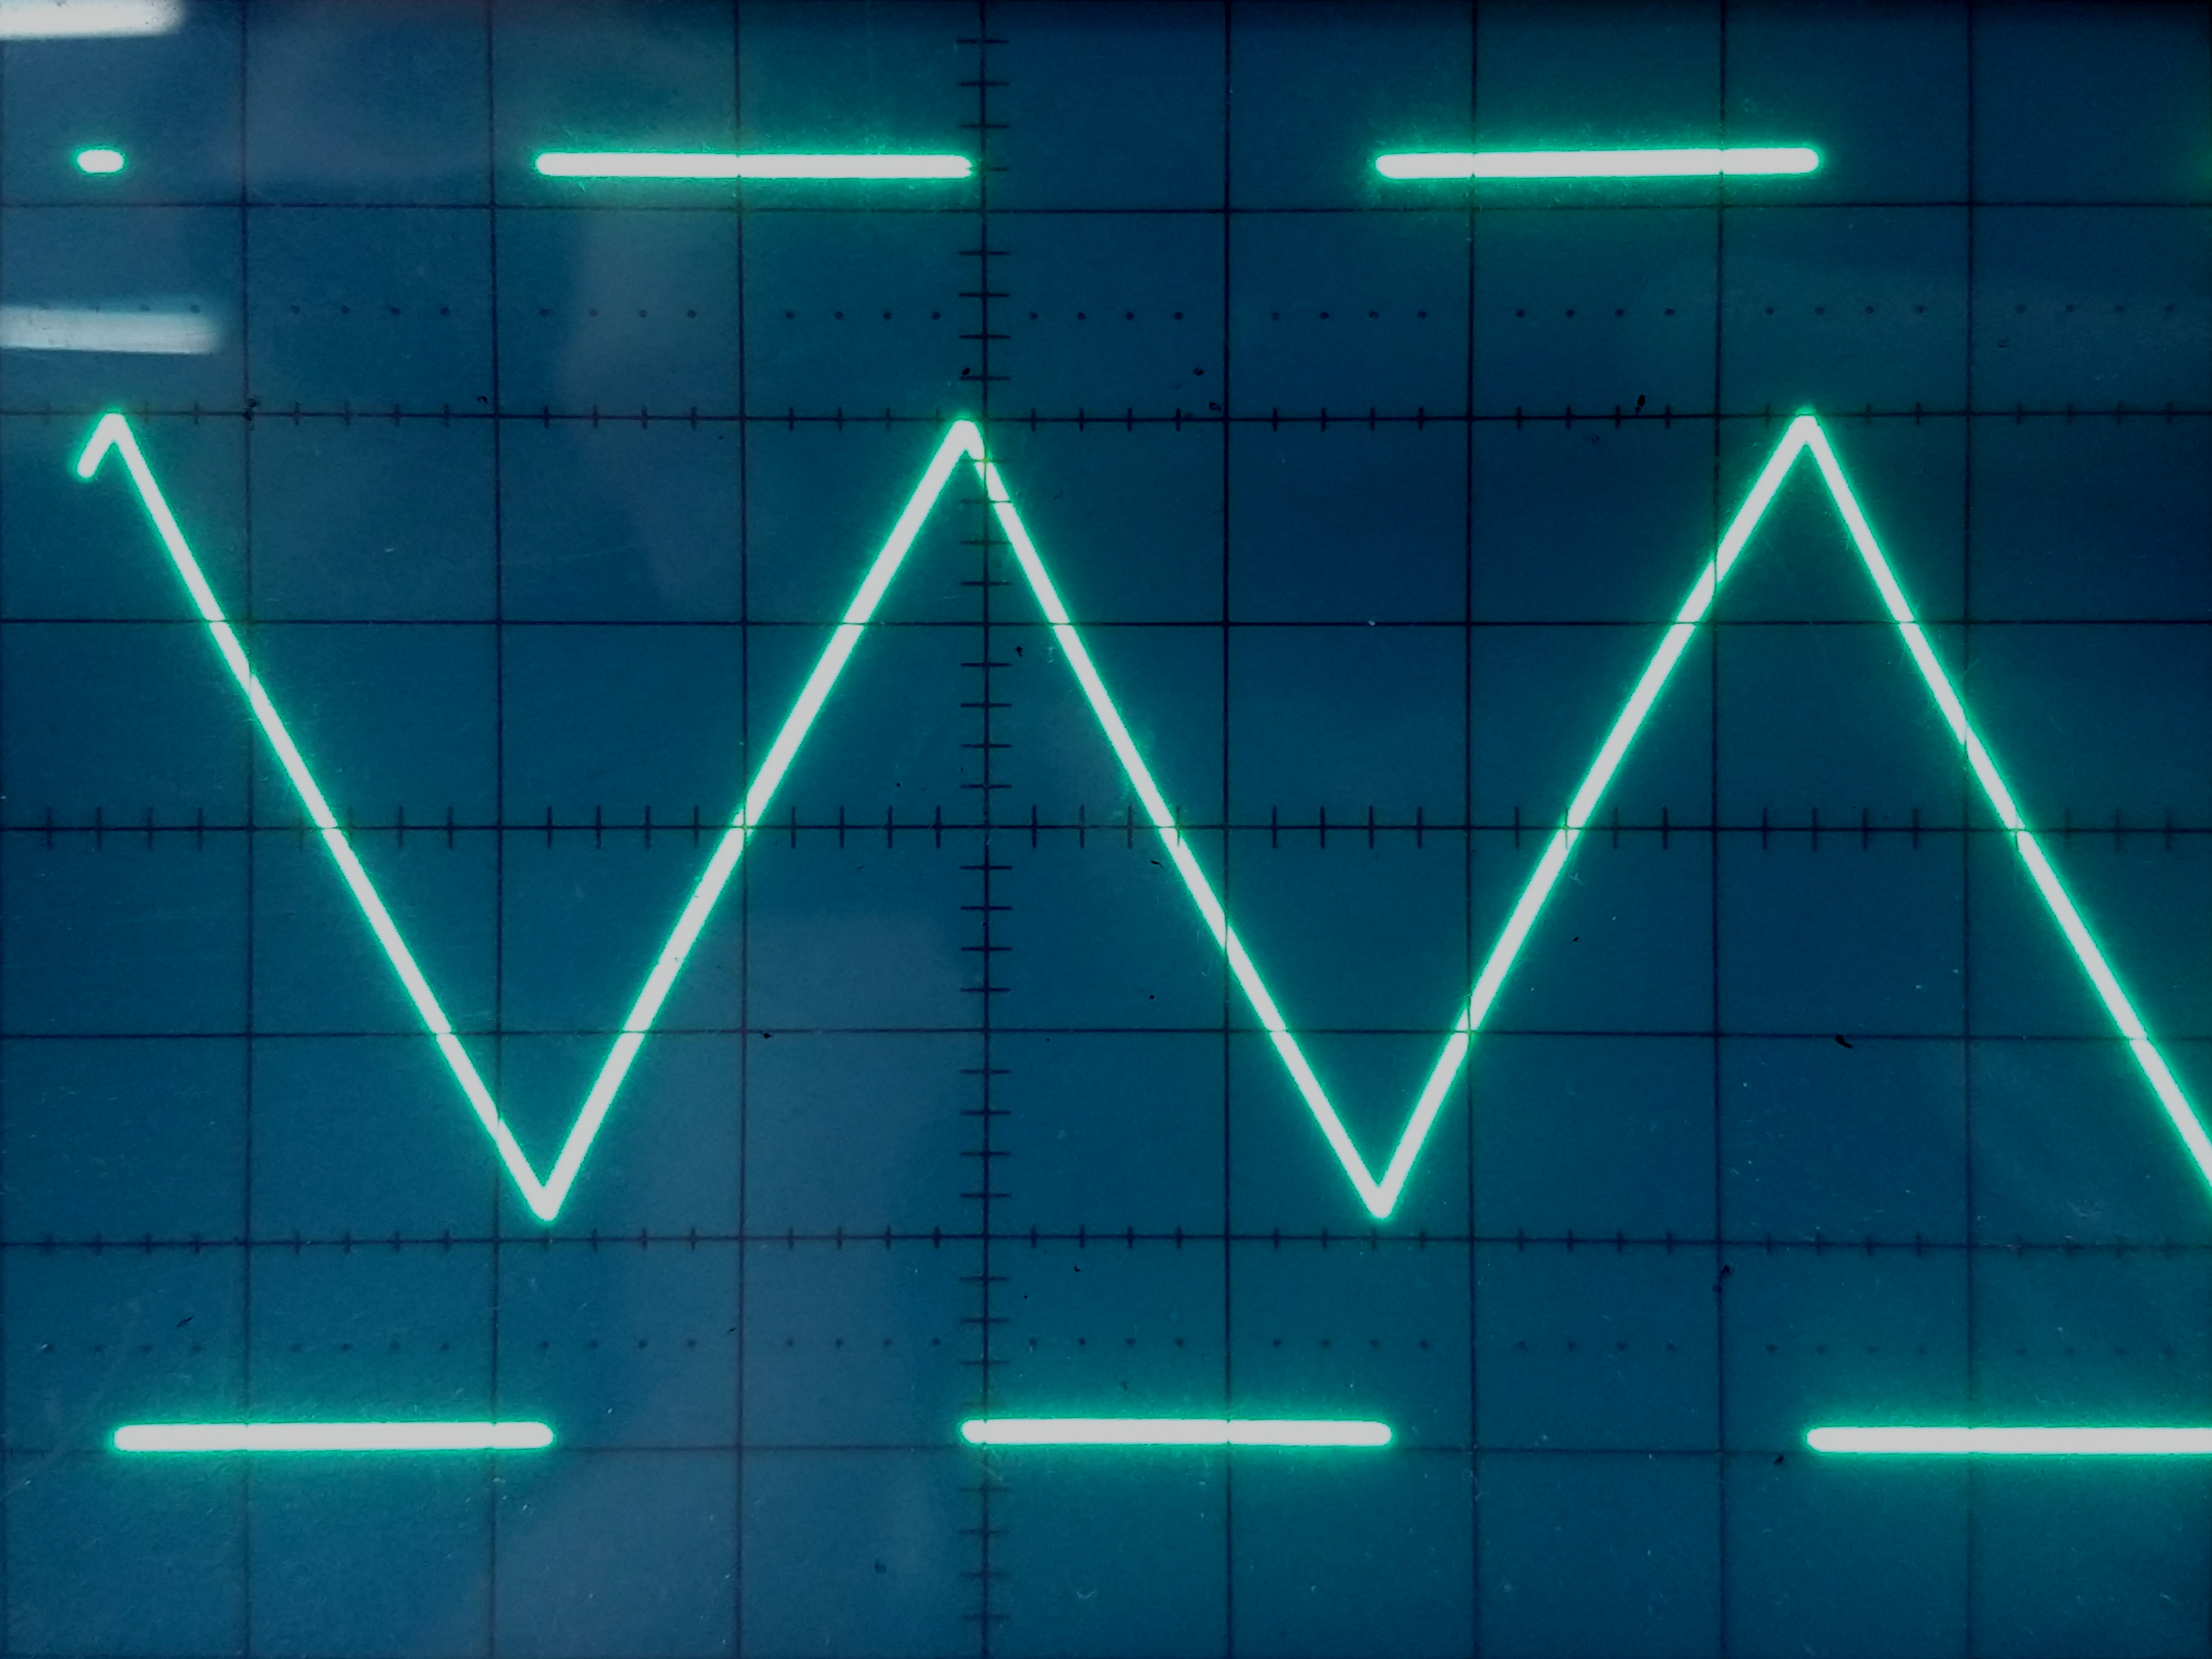
\includegraphics[width=4.5cm]{images/integrator-rechteck.jpg}
		\caption{Rechteckschwingung}
	\end{subfigure}
	~
	\begin{subfigure}[b]{0.3\textwidth}
		\centering
		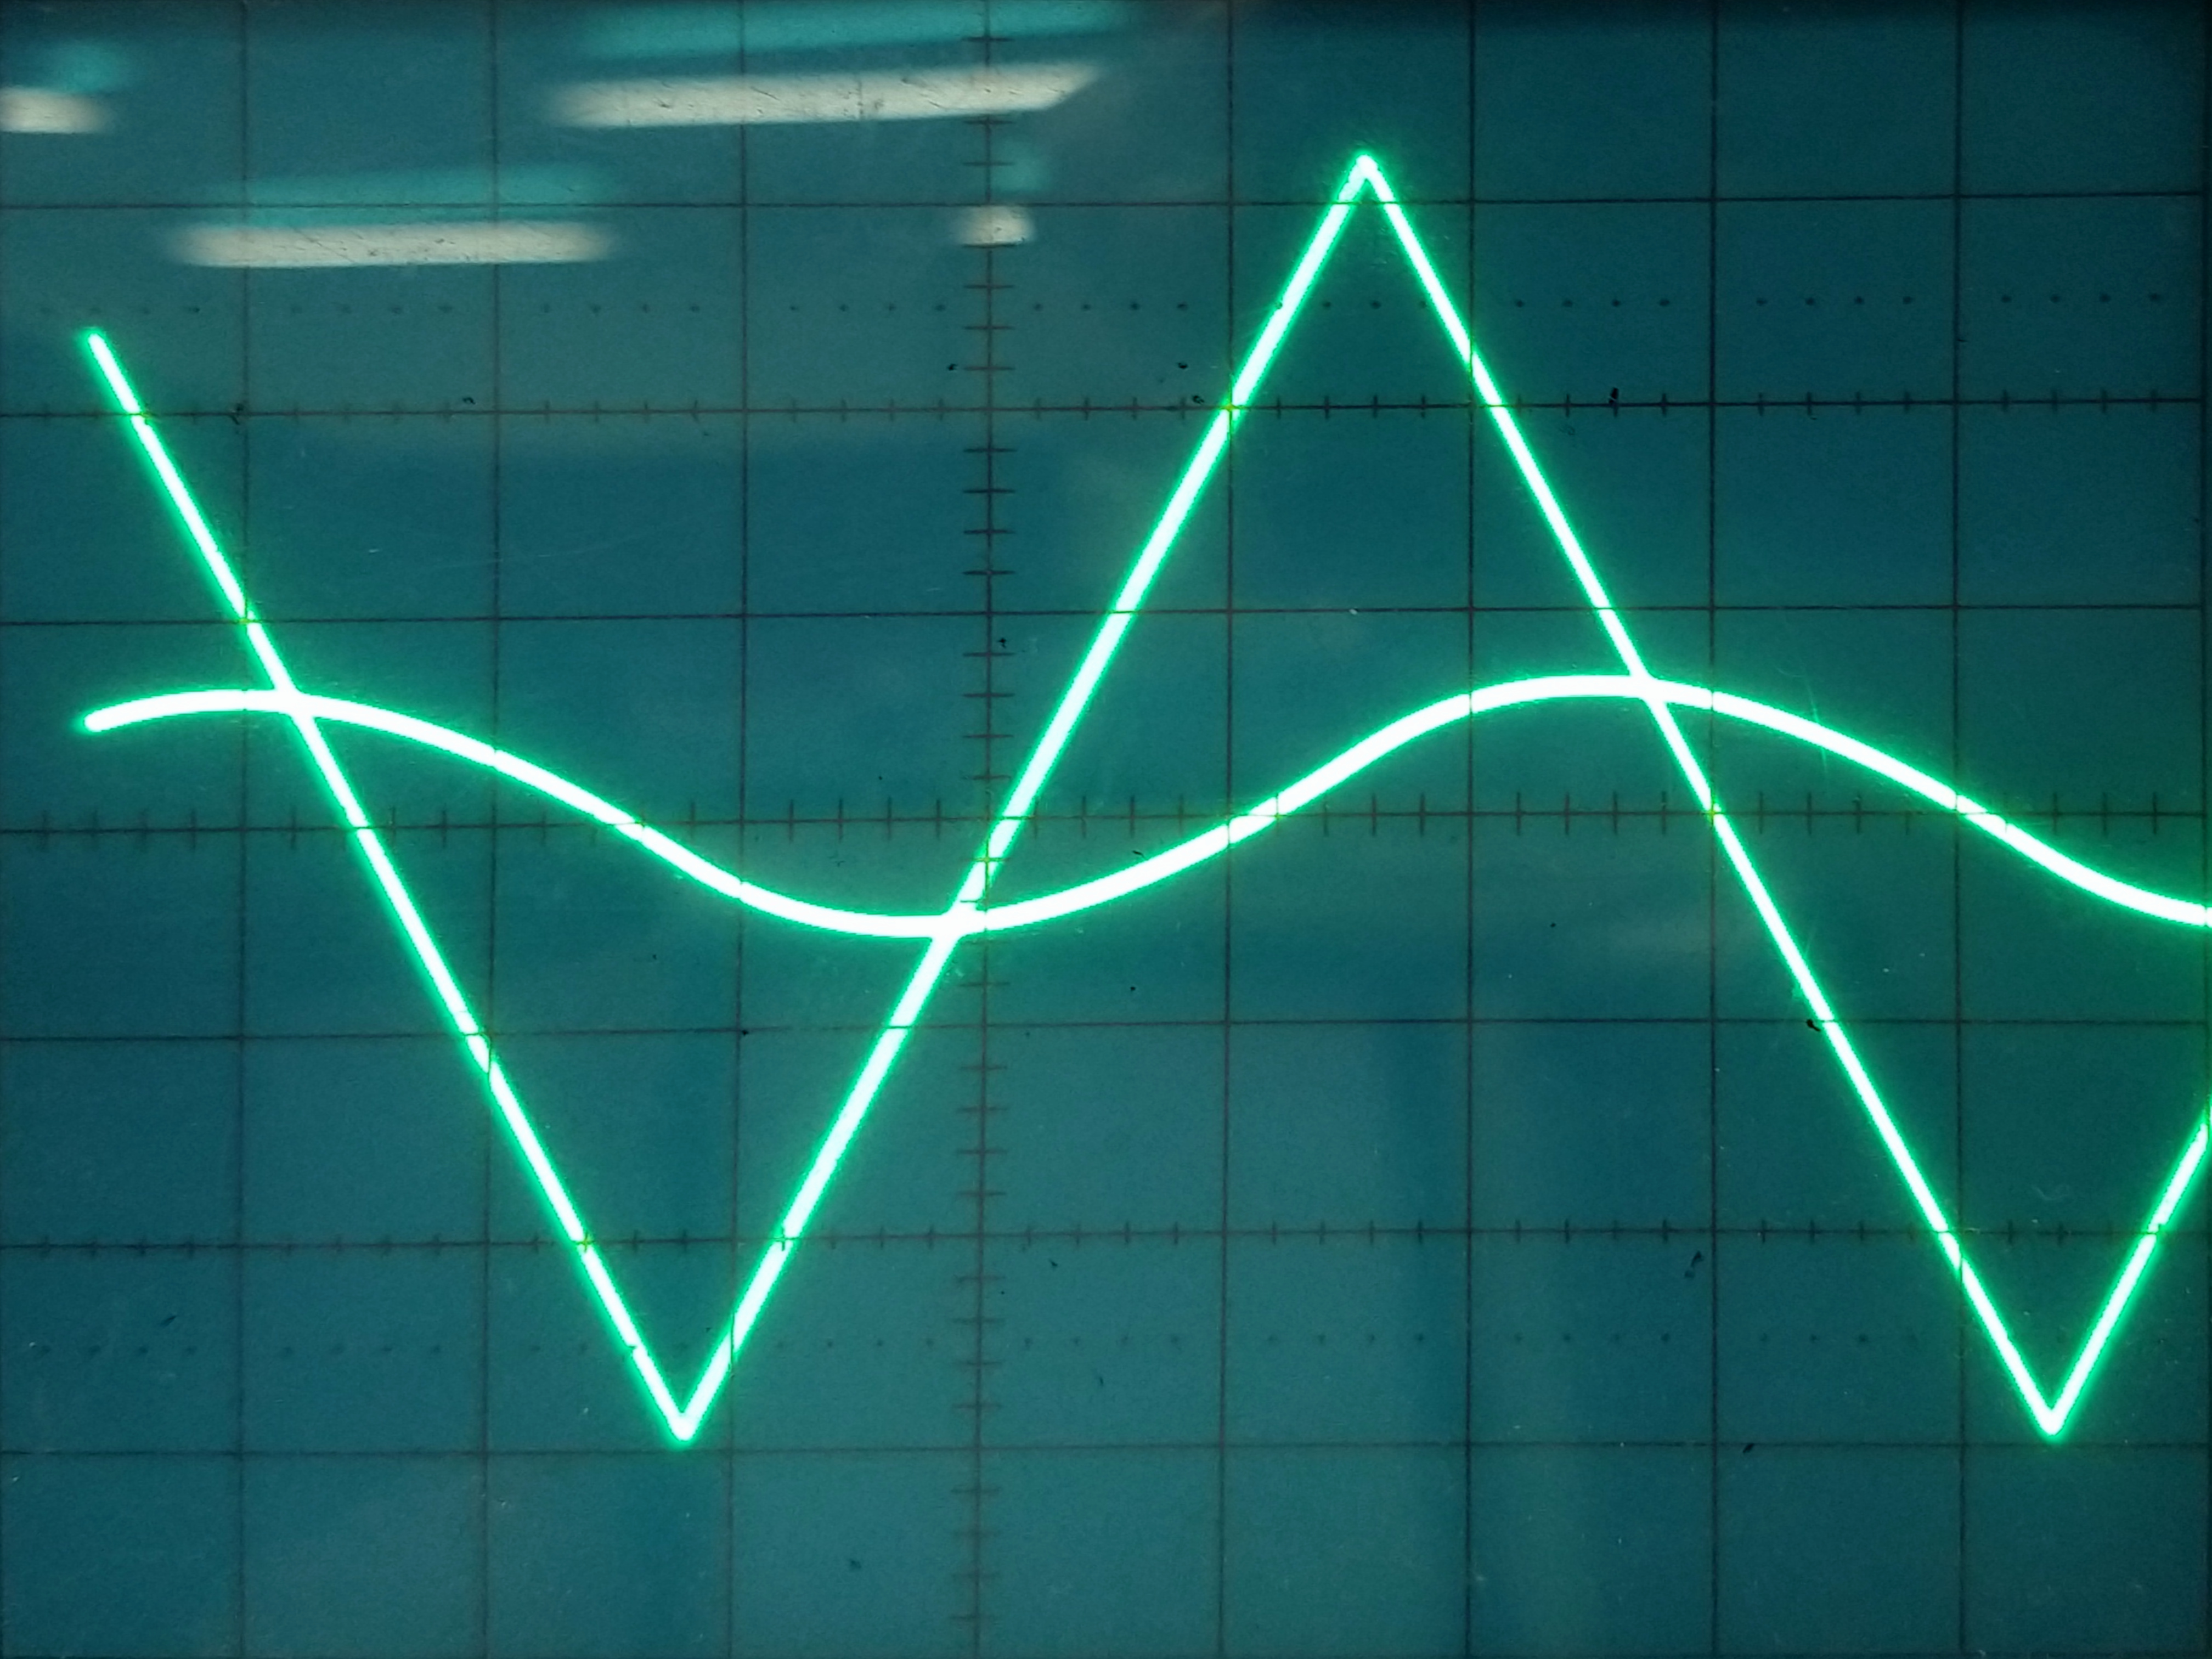
\includegraphics[width=4.5cm]{images/integrator-saegezahn.jpg}
		\caption{Dreieckschwingung}
	\end{subfigure}
	~
	\begin{subfigure}[b]{0.3\textwidth}
		\centering
		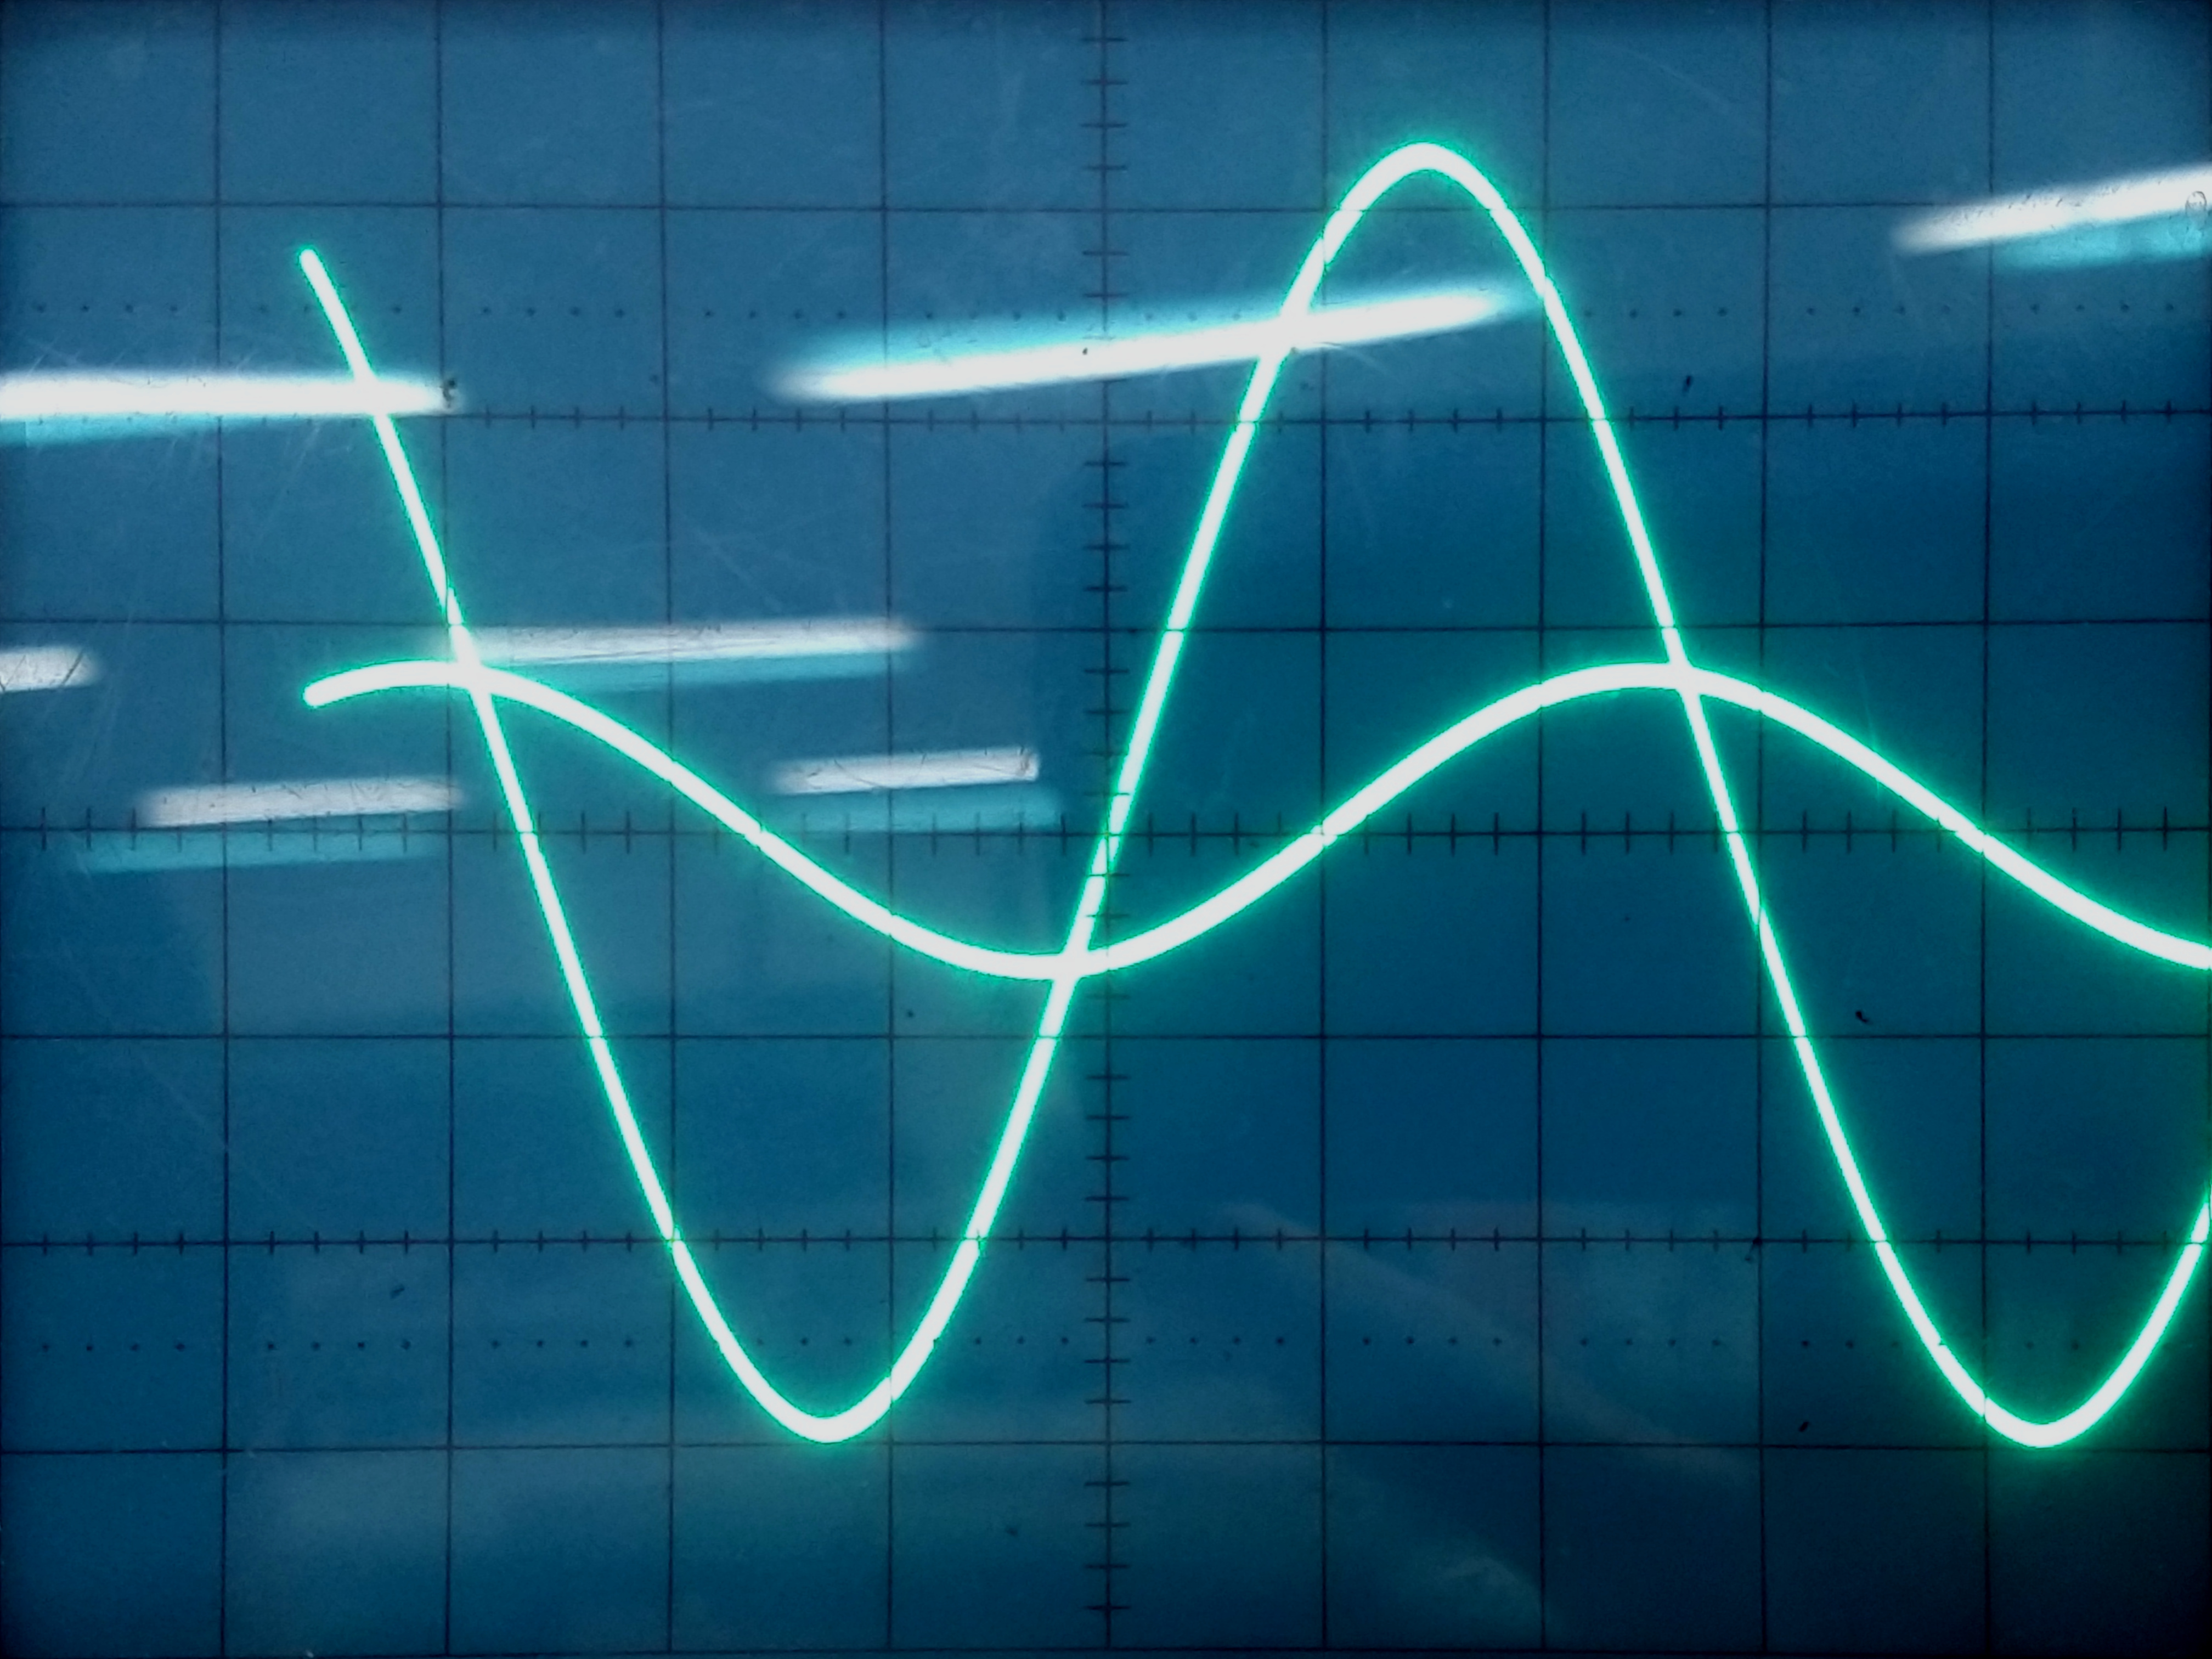
\includegraphics[width=4.5cm]{images/integrator-sinus.jpg}
		\caption{Sinus-Schwingung}
	\end{subfigure}
\end{figure}
